\documentclass[9pt]{pnas-new}
% Use the lineno option to display guide line numbers if required.
% Note that the use of elements such as single-column equations
% may affect the guide line number alignment. 

% \RequirePackage[english,slovene]{babel} % when writing in slovene
\RequirePackage[slovene,english]{babel} % when writing in english

% Custom added packages
\usetikzlibrary{shapes.geometric}

\templatetype{pnasresearcharticle} % Choose template 
% {pnasresearcharticle} = Template for a two-column research article
% {pnasmathematics} = Template for a one-column mathematics article
% {pnasinvited} = Template for a PNAS invited submission

\selectlanguage{english}
%\etal{in sod.} % comment out when writing in english
%\renewcommand{\Authands}{ in } % comment out when writing in english
%\renewcommand{\Authand}{ in } % comment out when writing in english

\newcommand{\set}[1]{\ensuremath{\mathbf{#1}}}
\renewcommand{\vec}[1]{\ensuremath{\mathbf{#1}}}
\newcommand{\uvec}[1]{\ensuremath{\hat{\vec{#1}}}}
\newcommand{\const}[1]{{\ensuremath{\kappa_\mathrm{#1}}}} 

\newcommand{\num}[1]{#1}

\graphicspath{{./fig/}}

\title{Predator-Prey Simulation Using Boids Model}

% Use letters for affiliations, numbers to show equal authorship (if applicable) and to indicate the corresponding author
\author{Matija Ojo}
\author{Miha Krajnc}
\author{Marko Adžaga}
\author{Janez Kuhar}

\affil{Collective behaviour course research seminar report} 

% Please give the surname of the lead author for the running footer
\leadauthor{Ojo} 

\selectlanguage{english}

% Please add here a significance statement to explain the relevance of your work
\significancestatement{Procedural generation of a tropic island and \\coral reef}{In computer graphics there is frequent need for displaying large vistas of natural looking terrain. Designing such terrain by hand is typically time consuming. With procedural generation, on the other hand, larger areas of natural looking terrain can be generated with or without minimal intervention in a relatively short time. In this work we present a process of procedural generation of a tropical island with the associated corral reef. We start by generating a heightmap for the base terrain. The heightmap is then transformed by simulating the processes of hydraulic and thermal erosion to achieve a more natural look of the terrain. As coral reefs often grow around tropical islands, we also simulate their growth as part of the last step. Real-time visualization is enabled during the simulation, so that one can observe the evolution of the terrain. Here we dynamically apply textures to the terrain based on its local characteristics. The result is a natural looking model of the textured tropical island and corral reef.}{Procedural generation | Terrain generation | Thermal and hydraulic erosion | Coral reef | Simulation | GPU}

\selectlanguage{english}

% Please include corresponding author, author contribution and author declaration information
%\authorcontributions{Please provide details of author contributions here.}
%\authordeclaration{Please declare any conflict of interest here.}
%\equalauthors{\textsuperscript{1}A.O.(Author One) and A.T. (Author Two) contributed equally to this work (remove if not applicable).}
%\correspondingauthor{\textsuperscript{2}To whom correspondence should be addressed. E-mail: author.two\@email.com}

% Keywords are not mandatory, but authors are strongly encouraged to provide them. If provided, please include two to five keywords, separated by the pipe symbol, e.g:
\keywords{Collective Behaviour | Boids | Simulation | Prey-Predator | Escape patterns } 

\begin{abstract}
% TODO
\nocite{papadopoulou2022emergence}
ToDo: Add abstract.
\end{abstract}

\dates{\textbf{\today}}
\program{BM-RI}
\vol{2023/24}
\no{CB:Group B} % group ID
%\fraca{FRIteza/201516.130}

\begin{document}

% Optional adjustment to line up main text (after abstract) of first page with line numbers, when using both lineno and twocolumn options.
% You should only change this length when you've finalised the article contents.
\verticaladjustment{-2pt}

\maketitle
\thispagestyle{firststyle}
\ifthenelse{\boolean{shortarticle}}{\ifthenelse{\boolean{singlecolumn}}{\abscontentformatted}{\abscontent}}{}

\section*{Introduction}

% If your first paragraph (i.e. with the \dropcap) contains a list environment (quote, quotation, theorem, definition, enumerate, itemize...), the line after the list may have some extra indentation. If this is the case, add \parshape=0 to the end of the list environment.
\dropcap{I}n 1987, Reynolds \cite{reynolds1987flocks} proposed a simple algorithm to model the
flocking behavior of birds, herding of sheep, and similar phenomena, known as the Boids (Bird-oid objects) model.
In contrast to controlling the interactions of the entire flock, the Boids simulation focuses on
dictating the behavior of each individual boid. Despite consisting of a few simple rules, this
algorithm produces complex and lifelike behaviors similar to those observed in nature.

\noindent Every boid abides by three simple rules:
\begin{enumerate}
	\item Avoid collisions.
	      \begin{center}
		      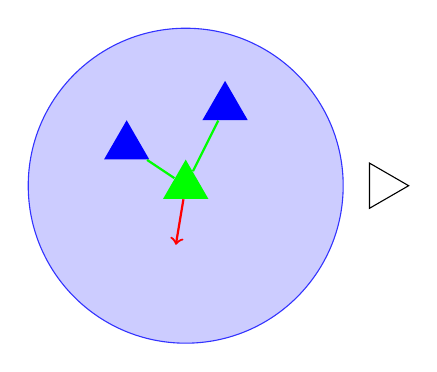
\begin{tikzpicture}
			      % Draw a semi-transparent blue circle with a dark border
			      \draw[fill=blue!20, draw=blue!80] (0,0) circle (2);
			      % Define a triangle shape
			      \node[regular polygon, regular polygon sides=3, minimum size=.5cm, fill,green] (t1) at (0,0) {};
			      \node[regular polygon, regular polygon sides=3, minimum size=.5cm, fill,blue] (t2) at (.5, 1) {};
			      \node[regular polygon, regular polygon sides=3, minimum size=.5cm, fill,blue] (t3) at (-.75, .5) {};
			      % Outside,rotated
			      \node[regular polygon, regular polygon sides=3, minimum size=.5cm, draw, rotate=30] (rotated) at (2.5,0) {};

			      \draw[green,thick] (t1) -- (t2);
			      \draw[green,thick] (t1) -- (t3);

			      \draw[red,thick,->] (t1) -- (-.125,-.75);
		      \end{tikzpicture}
	      \end{center}
	\item Maintain the same heading and speed as the neighboring boids.
	      \begin{center}
		      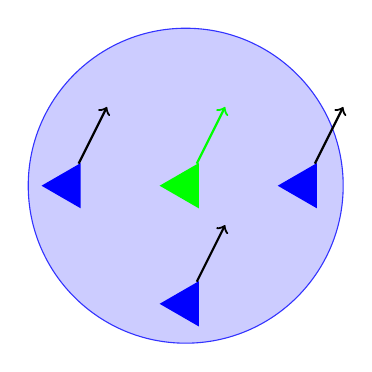
\begin{tikzpicture}
			      % Draw a semi-transparent blue circle with a dark border
			      \draw[fill=blue!20, draw=blue!80] (0,0) circle (2);
			      % Define a triangle shape
			      \node[regular polygon, regular polygon sides=3, minimum size=.5cm, fill,green,rotate=-30] (t1) at (0,0) {};
			      \node[regular polygon, regular polygon sides=3, minimum size=.5cm, fill,blue,rotate=-30] (t2) at (-1.5, 0) {};
			      \node[regular polygon, regular polygon sides=3, minimum size=.5cm, fill,blue,rotate=-30] (t3) at (1.5, 0) {};
			      \node[regular polygon, regular polygon sides=3, minimum size=.5cm, fill,blue,rotate=-30] (t4) at (0, -1.5) {};

			      \draw[green,thick,->] (t1) -- ++(.5, 1);
			      \draw[black,thick,->] (t2) -- ++(.5, 1);
			      \draw[black,thick,->] (t3) -- ++(.5, 1);
			      \draw[black,thick,->] (t4) -- ++(.5, 1);
		      \end{tikzpicture}
	      \end{center}
	\item Gravitate toward the center of the flock.
	      \begin{center}
		      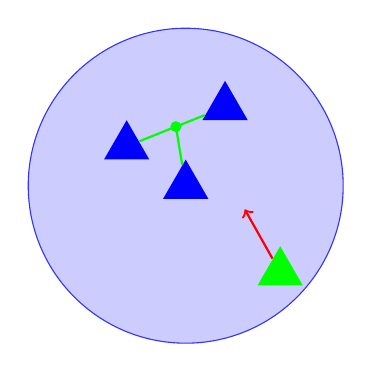
\begin{tikzpicture}
			      % Draw a semi-transparent blue circle with a dark border
			      \draw[fill=blue!20, draw=blue!80] (0,0) circle (2);
			      % Define a triangle shape
			      \node[regular polygon, regular polygon sides=3, minimum size=.5cm, fill,blue] (t1) at (0,0) {};
			      \node[regular polygon, regular polygon sides=3, minimum size=.5cm, fill,blue] (t2) at (.5, 1) {};
			      \node[regular polygon, regular polygon sides=3, minimum size=.5cm, fill,blue] (t3) at (-.75, .5) {};

			      \node[regular polygon, regular polygon sides=3, minimum size=.5cm, fill,green] (t4) at (1.2, -1.1) {};

			      \draw[green, thick] (t1) -- (-.125,.75);
			      \fill[green, thick] (-.125,.75) circle (2pt);
			      \draw[green,thick] (t2) -- (t3);

			      \draw[red,thick,->] (t4) -- (.75,-.3);
		      \end{tikzpicture}
	      \end{center}
\end{enumerate}

We will present how we implemented such Boid simulation, with an additional step which will make simulating different Boids (prey, predator) easier.
% TODO: We should also include logic for predator (if we implement it for this milestone)

\section*{Methods}
ToDo: Add Methods.
\section*{Results}
ToDo: Add Results.
\section*{Discussion}
ToDo: Conclusion/Discussion.
\acknow{ToDo: division of work.}
\showacknow % Display the acknowledgments section

% \pnasbreak splits and balances the columns before the references.
% If you see unexpected formatting errors, try commenting out this line
% as it can run into problems with floats and footnotes on the final page.
%\pnasbreak

\begin{multicols}{2}
	\section*{\bibname}
	% Bibliography
	\bibliography{./bib/bibliography}
\end{multicols}

\end{document}